% main.tex — academic article assembled by the Phase 5 pipeline.
% Build engine: lualatex (NOT pdflatex) — required for fontspec + Hebrew BiDi.
% Bibliography:  biblatex with the biber backend.
% Build order:   lualatex -> biber -> lualatex -> lualatex
\documentclass[11pt,a4paper]{report}

% ── Fonts & languages (LuaLaTeX) ────────────────────────────────────────────
\usepackage{fontspec}
\usepackage{polyglossia}
\setmainlanguage{english}
\setotherlanguage{hebrew}
\setmainfont{Latin Modern Roman}
% A Hebrew-capable font (Culmus "David CLM" ships with TeX Live). Swap this
% for any installed Hebrew font if David CLM is unavailable on the build host.
\newfontfamily\hebrewfont[Script=Hebrew]{David CLM}

% ── Mathematics ─────────────────────────────────────────────────────────────
\usepackage{amsmath}
\usepackage{amssymb}

% ── Graphics & tables ───────────────────────────────────────────────────────
\usepackage{graphicx}
\usepackage{booktabs}
\graphicspath{{../figures/}{figures/}}

% ── Headers & footers (every body page) ─────────────────────────────────────
\usepackage{fancyhdr}
\pagestyle{fancy}
\fancyhf{}
\fancyhead[L]{From RNN and LSTM to Transformers and AI Agents}
\fancyhead[R]{\thepage}
\fancyfoot[C]{Course 203.3763 — Orchestration of AI Agents}
\renewcommand{\headrulewidth}{0.4pt}
\renewcommand{\footrulewidth}{0.4pt}

% ── Bibliography (biblatex + biber) ─────────────────────────────────────────
\usepackage[backend=biber,style=numeric,sorting=nyt]{biblatex}
\addbibresource{references.bib}

% ── Hyperlinks (load late) ──────────────────────────────────────────────────
\usepackage[hidelinks]{hyperref}
\hypersetup{
  pdftitle={From RNN and LSTM to Transformers and AI Agents},
  pdfsubject={Course 203.3763 — Orchestration of AI Agents},
  colorlinks=true,
  linkcolor=blue!50!black,
  citecolor=green!40!black,
  urlcolor=blue!60!black
}

% ── Document metadata (filled by the title page) ────────────────────────────
\newcommand{\coursenumber}{203.3763}
\newcommand{\coursename}{Orchestration of AI Agents}
\newcommand{\lecturername}{Dr.\ Yoram Reuven Segal}
% Student name is a placeholder: replace before submission.
\newcommand{\studentname}{[STUDENT NAME — replace before submission]}

\begin{document}
% ===== TITLE PAGE (F2) =====
\begin{titlepage}
  \centering
  \vspace*{2cm}
  {\Huge\bfseries From RNN and LSTM to\\[0.3em] Transformers and AI Agents\par}
  \vspace{0.6cm}
  {\Large\itshape How Modern AI Systems Generate Knowledge\par}
  \vspace{2cm}
  \begin{tabular}{rl}
    \textbf{Course}   & \coursenumber\ — \coursename \\[0.4em]
    \textbf{Lecturer} & \lecturername \\[0.4em]
    \textbf{Student}  & \studentname \\[0.4em]
    \textbf{Date}     & \today \\
  \end{tabular}
  \vfill
  {\small Assembled by a CrewAI multi-agent pipeline and typeset with LuaLaTeX.\par}
\end{titlepage}
\pagenumbering{roman}

% ===== ABSTRACT (F13) =====
\chapter*{Abstract}
\addcontentsline{toc}{chapter}{Abstract}
This article traces the evolution of sequence modelling in modern artificial
intelligence: from recurrent neural networks (RNNs) and their long
short-term memory (LSTM) refinement, through the attention mechanism and the
Transformer architecture, to the multi-agent systems that orchestrate them.
We explain why recurrent models were originally needed, how gating addressed
the vanishing-gradient problem, and why scaled dot-product attention enabled
parallel, long-range context modelling. We then connect attention and context
to agentic systems, using the CrewAI framework as an example of role-based
orchestration. The document itself was assembled by such a pipeline, and
serves as a worked example of how a team of cooperating agents can research,
write, illustrate, and typeset an academic PDF end to end.

% ===== TABLE OF CONTENTS (F3) =====
\tableofcontents
\cleardoublepage
\pagenumbering{arabic}

% ===== BODY CHAPTERS (F4) =====
\chapter{Introduction}
Sequence data — language, audio, time series — is everywhere, and modelling it
well has driven much of modern AI. This article follows that thread from early
recurrent models to the Transformer and on to multi-agent orchestration. The
core mechanism that unifies the later chapters, scaled dot-product attention,
is given in \autoref{eq:attention}, and the conceptual trade-offs between the
models are summarised in \autoref{tab:models} and \autoref{fig:complexity}.

\chapter{Recurrent Neural Networks (RNNs)}
Recurrent networks process a sequence one step at a time, maintaining a hidden
state that carries information forward~\cite{rumelhart1986}. This makes them a
natural fit for variable-length input, but the same step-by-step recurrence
makes long-range dependencies hard to learn: gradients propagated through many
time steps tend to vanish or explode~\cite{bengio1994}, limiting how far back
the model can effectively remember.

\chapter{Long Short-Term Memory (LSTM)}
The LSTM addresses the vanishing-gradient problem with a gated cell
state~\cite{hochreiter1997}. Input, forget, and output gates regulate what is
written to, retained in, and read from the cell, letting error signals flow
across many steps without decaying. Gated recurrent units later offered a
lighter variant of the same idea~\cite{cho2014}. These models substantially
extended the usable memory horizon, yet remained fundamentally sequential.

\chapter{Transformers and Attention}
Attention let a model align directly with any position in the
input~\cite{bahdanau2015}, and the Transformer removed recurrence entirely in
favour of self-attention~\cite{vaswani2017}. The scaled dot-product attention
operation is:
\begin{equation}
  \operatorname{Attention}(Q, K, V)
    = \operatorname{softmax}\!\left(\frac{Q K^{\top}}{\sqrt{d_k}}\right) V
  \label{eq:attention}
\end{equation}
Each query in $Q$ is scored against every key in $K$; dividing by $\sqrt{d_k}$
keeps the scores from saturating the \texttt{softmax}, whose weights then form
a context-aware combination of the values $V$. Because every position attends
to every other in parallel, the maximum dependency path is constant rather
than linear in the sequence length, as \autoref{fig:complexity} illustrates.
This design also underpins large pre-trained encoders such as
BERT~\cite{devlin2019}.

\begin{figure}[ht]
  \centering
  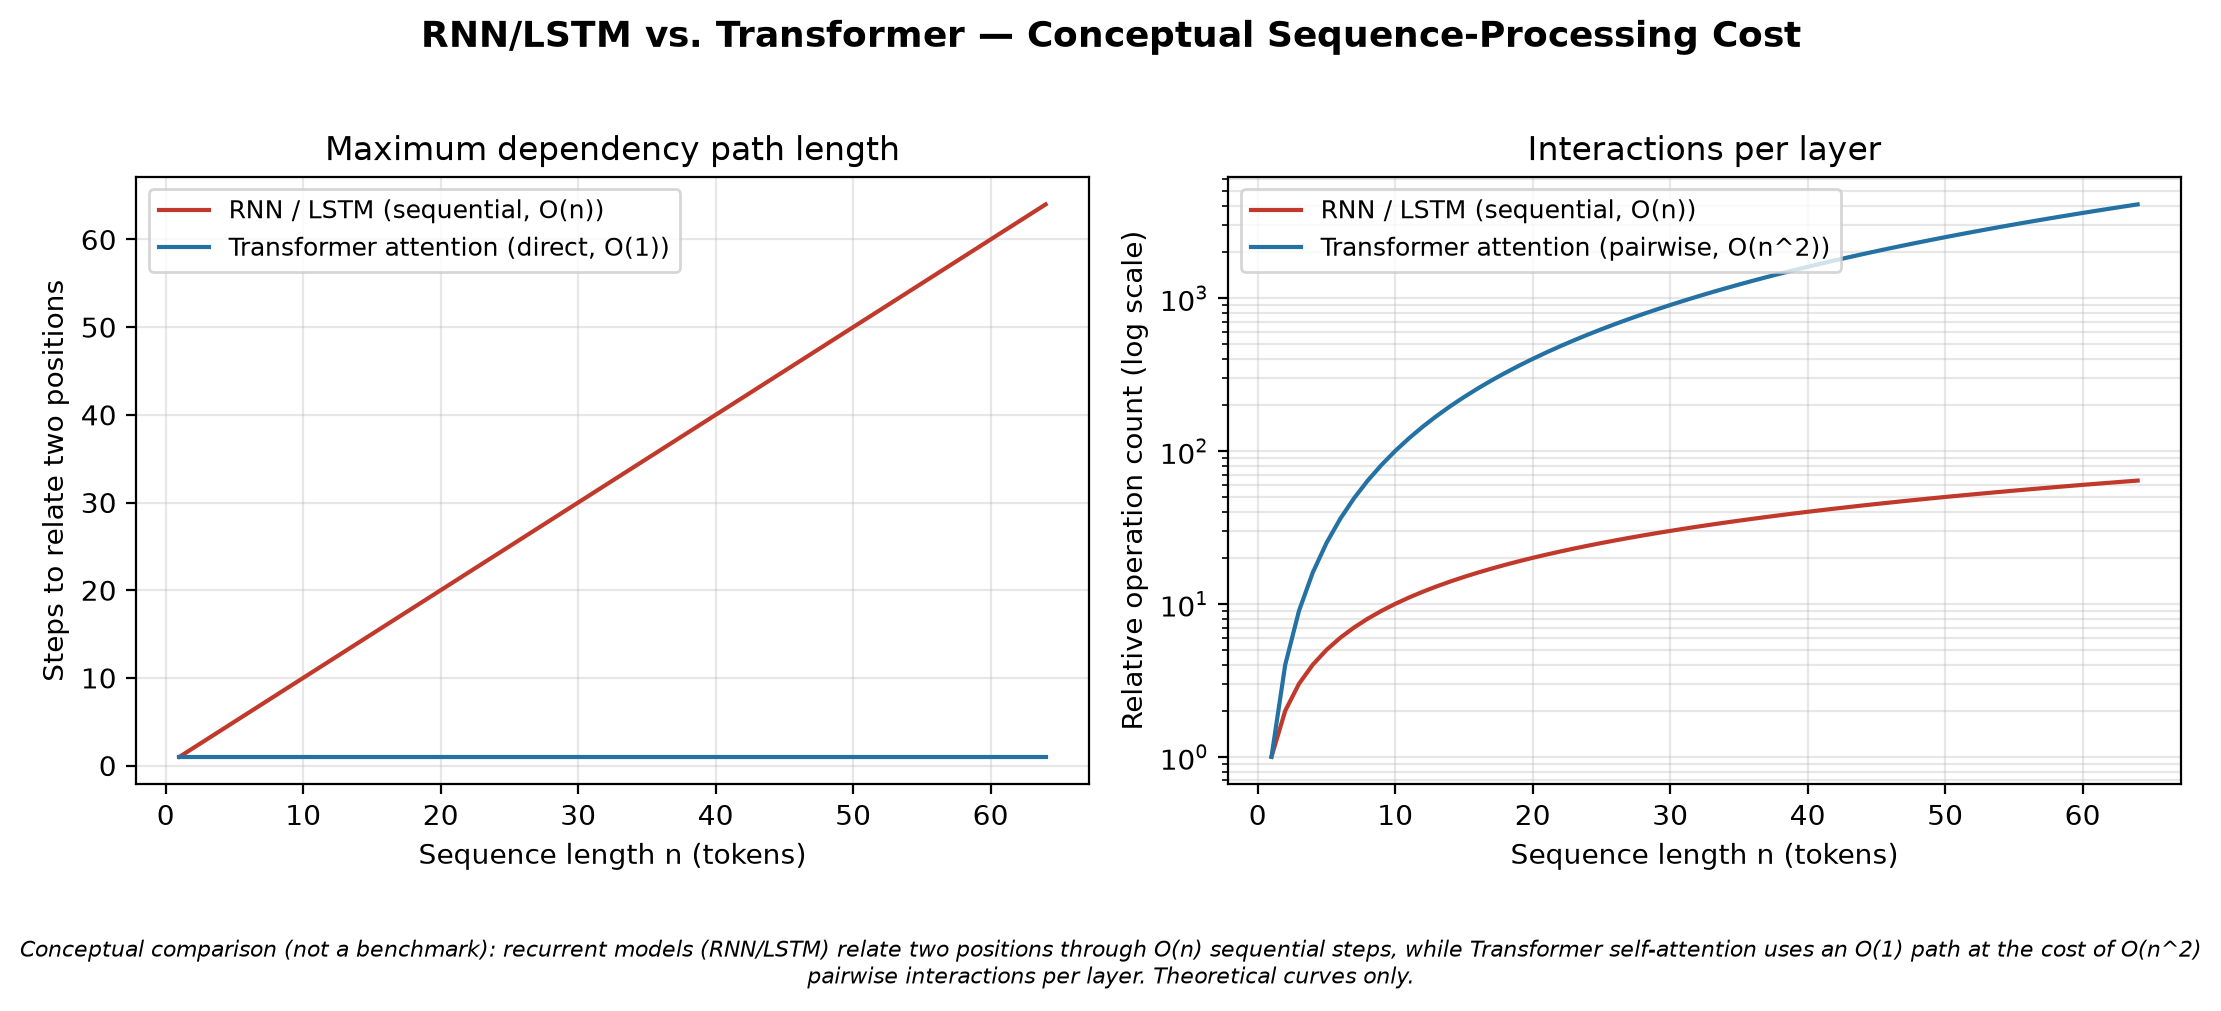
\includegraphics[width=0.85\textwidth]{complexity_comparison.png}
  \caption{Conceptual comparison of the maximum dependency path length for
    recurrent models (linear in sequence length) versus Transformer
    self-attention (constant). Theoretical illustration, not a benchmark.}
  \label{fig:complexity}
\end{figure}

\chapter{AI Agents and CrewAI}
Attention gives a model context within a single forward pass; agentic systems
extend the same idea across time and tools. The CrewAI framework organises
large-language-model agents into roles with explicit goals and shared context,
running them as a sequential or hierarchical process. The output of one agent
becomes the context of the next, much as this document was produced. See the
\href{https://docs.crewai.com}{CrewAI documentation} for the framework's API.

\chapter{Comparison Table}
\autoref{tab:models} contrasts the mechanisms discussed above. It restates
established, course-aligned definitions; it contains no measured results.
\begin{table}[ht]
  \centering
  \caption{Conceptual comparison of recurrent models, the Transformer, and
    CrewAI agent orchestration.}
  \label{tab:models}
  \begin{tabular}{@{}llll@{}}
    \toprule
    \textbf{System} & \textbf{Core mechanism} & \textbf{Long-range} & \textbf{Parallelism} \\
    \midrule
    RNN          & Recurrent hidden state      & Weak (vanishing grad.) & Low  \\
    LSTM         & Gated cell state            & Improved via gating    & Low  \\
    Transformer  & Self-attention              & Strong (direct access) & High \\
    CrewAI agents& Roles + shared context      & Carried by task context& Orchestrated \\
    \bottomrule
  \end{tabular}
\end{table}

\chapter{Bilingual Chapter — Hebrew and English (BiDi)}
This chapter demonstrates bidirectional (BiDi) typesetting: left-to-right
English mixed with right-to-left Hebrew, handled by \texttt{polyglossia} under
LuaLaTeX. The Hebrew term for ``attention'' is \texthebrew{קשב}, and ``neural
network'' is \texthebrew{רשת עצבית}. A full Hebrew paragraph follows:
\begin{hebrew}
מנגנון הקשב (attention) מאפשר למודל להתמקד בחלקים הרלוונטיים של הקלט.
ארכיטקטורת הטרנספורמר מבססת את כל החישוב על מנגנון זה, ובכך מתגברת על מגבלות
הזיכרון של רשתות נשנות כגון RNN ו-LSTM. מערכות סוכנים כמו CrewAI מרחיבות את
רעיון ההקשר אל מעבר למודל בודד.
\end{hebrew}
The two scripts coexist in one chapter with correct directionality.

\chapter{Conclusion}
From RNNs to LSTMs to Transformers, each step lengthened the reach of context;
multi-agent orchestration carries that context across tools and tasks. The
references below ground every architectural claim in its original source.

% ===== BIBLIOGRAPHY (F11) =====
\printbibliography[heading=bibintoc,title={References}]
\end{document}
